\documentclass{article}

\usepackage{graphicx}
\usepackage{multirow}
\usepackage{amsmath,amssymb,amsfonts,amsthm, mathrsfs}
\usepackage[title]{appendix}
\usepackage{xcolor}
\usepackage{textcomp}
\usepackage{manyfoot, booktabs}
\usepackage{algorithm, algorithmicx, algpseudocode}
\usepackage{listings}
\usepackage{biblatex}

\usepackage[english]{babel}

\raggedbottom

\lstset{
    language=Python,                 
    basicstyle=\ttfamily\small,      
    keywordstyle=\color{blue},       
    stringstyle=\color{red},         
    commentstyle=\color{orange},      
    morecomment=[s][\color{gray}]{"""}{"""}, 
    numbers=left,                    
    numberstyle=\tiny\color{gray},   
    stepnumber=1,                    
    numbersep=10pt,                  
    backgroundcolor=\color{white},   
    showspaces=false,                
    showstringspaces=false,          
    showtabs=false,                  
    frame=single,                    
    captionpos=b,                    
    breaklines=true,                 
    breakatwhitespace=false,         
    tabsize=4,                       
    escapeinside={\%*}{*}           
}

\begin{document}

\title{1 day as ....\\ Red Bull Analysts\\Big Data Final Term Project}

\author{Enrique Ulises Báez Gómez Tagle \\ Sara Rocío Miranda Mateos \\ Mauricio Ascencio Martinez}

\maketitle

\begin{abstract}
This report encapsulates a comprehensive data-driven analysis aimed at enhancing the strategic decisions of the Red Bull Racing Team. Leveraging advanced data analytics, we scrutinize various aspects of Formula 1 racing, from pit stop efficiency to the reliability of car components across different race circuits. The insights garnered are intended to pinpoint potential areas for improvement, bolster race strategies, and augment overall team performance in the competitive realm of Formula 1.
\end{abstract}

\tableofcontents
\newpage

\section{Introduction}
The realm of Formula 1 is not just a test of speed but a colossal data battleground where each decision is crucial for success. This report, crafted during a day's stint as data analysts for Red Bull Racing, harnesses the power of big data to unfold patterns and anomalies that influence race outcomes. By analyzing data from recent seasons and the current 2024 season, we aim to uncover actionable insights that can refine race strategies, enhance car reliability, and optimize performance. From evaluating pit stop strategies to analyzing circuit-specific performance, our analysis is tailored to empower Red Bull Racing with the intelligence to make informed strategic decisions.


\section{Infrastructure / Architecture}

\begin{itemize}
    \item \textbf{Data Lakehouse Configuration:} Central to our project is a Data Lakehouse architecture designed for scalability and resilience within an AWS environment. This setup includes multiple layers of data storage and processing capabilities, ensuring efficient data management and analysis.
    
    \item \textbf{Storage Layers:} 
        \begin{itemize}
            \item \textbf{Raw Data Storage (RAW Layer):} Utilizes Amazon S3 to store unprocessed, raw data ingested from various sources.
            \item \textbf{Cleansed Data Storage (Cleansed Layer):} Stores cleaned and transformed data in Amazon S3, ready for further analysis.
            \item \textbf{Data Warehouse Storage (Data Warehouse Layer):} Contains structured and optimized data in Amazon S3, prepared for querying and visualization.
        \end{itemize}
    
    \item \textbf{Data Ingestion:} 
        \begin{itemize}
            \item \textbf{Real-Time Data Ingestion (AWS Lambda):} Handles the real-time ingestion of data, storing it in the RAW Layer.
            \item \textbf{Batch Data Ingestion (Static Dataset):} Manages the batch ingestion of static datasets, such as CSV files, into the RAW Layer.
        \end{itemize}
    
    \item \textbf{Data Transformation:} 
        \begin{itemize}
            \item \textbf{ETL Processing Jobs (AWS Glue):} Performs ETL (Extract, Transform, Load) operations to clean and transform data from the RAW Layer to the Cleansed Layer.
        \end{itemize}
    
    \item \textbf{Data Analysis:} 
        \begin{itemize}
            \item \textbf{Data Analytics and Processing (AWS EMR):} Utilizes Amazon EMR to run advanced data processing and analytical tasks on data from the Cleansed Layer, producing structured results stored in the Data Warehouse Layer.
        \end{itemize}
    
    \item \textbf{Data Cataloging:} 
        \begin{itemize}
            \item \textbf{Metadata Management (AWS Glue Data Catalog):} Catalogs the metadata of datasets in the Cleansed Layer, facilitating efficient data discovery and access.
        \end{itemize}
    
    \item \textbf{Data Visualization:} 
        \begin{itemize}
            \item \textbf{Visualization and Analysis (RStudio):} Processes the curated datasets in the Data Warehouse Layer locally to create insightful visualizations and analysis, supporting decision-making.
        \end{itemize}
    
    \item \textbf{Deployment Process:}
        \begin{enumerate}
            \item We initiated our deployment by setting up the AWS CLI, enabling us to interact with AWS services seamlessly.
            \item Amazon S3 buckets were created to host our data layers, carefully chosen to be in proximity to our compute resources to minimize latency.
            \item For infrastructure provisioning, we utilized both AWS CloudFormation and Terraform. AWS CloudFormation was used for managing AWS-specific resources, ensuring consistent and repeatable deployments within the AWS ecosystem. Terraform was employed for managing multi-cloud resources and ensuring infrastructure as code principles across various environments.
            \item AWS Glue was configured to automate our ETL processes, facilitating efficient data transformation and loading into our cleansed and data warehouse layers.
            \item Amazon EMR clusters were set up for big data processing, with configurations tailored to optimize performance and cost.
            \item Continuous Integration and Continuous Deployment (CI/CD) pipelines were implemented using AWS CodePipeline and Jenkins, automating the deployment process and ensuring that updates to our infrastructure and applications could be rolled out smoothly.
            \item Monitoring and logging were established using Amazon CloudWatch and AWS CloudTrail, providing real-time insights and audit trails for all activities within our environment.
            \item Security best practices were followed, including the use of IAM roles and policies to control access, as well as encryption of data at rest and in transit to protect our sensitive information.
        \end{enumerate}
    
\end{itemize}

This infrastructure is pivotal to our project, allowing us to effectively utilize big data technologies to derive valuable insights from the Formula 1 dataset. The design prioritizes scalability, efficiency, and cost-effectiveness, ensuring it meets the high demands of large-scale data processing and analysis. 

Ultimately, this setup empowers us to make data-driven decisions that enhance our understanding and strategic planning within the context of Formula 1.

\begin{figure}[H]
    \centering
    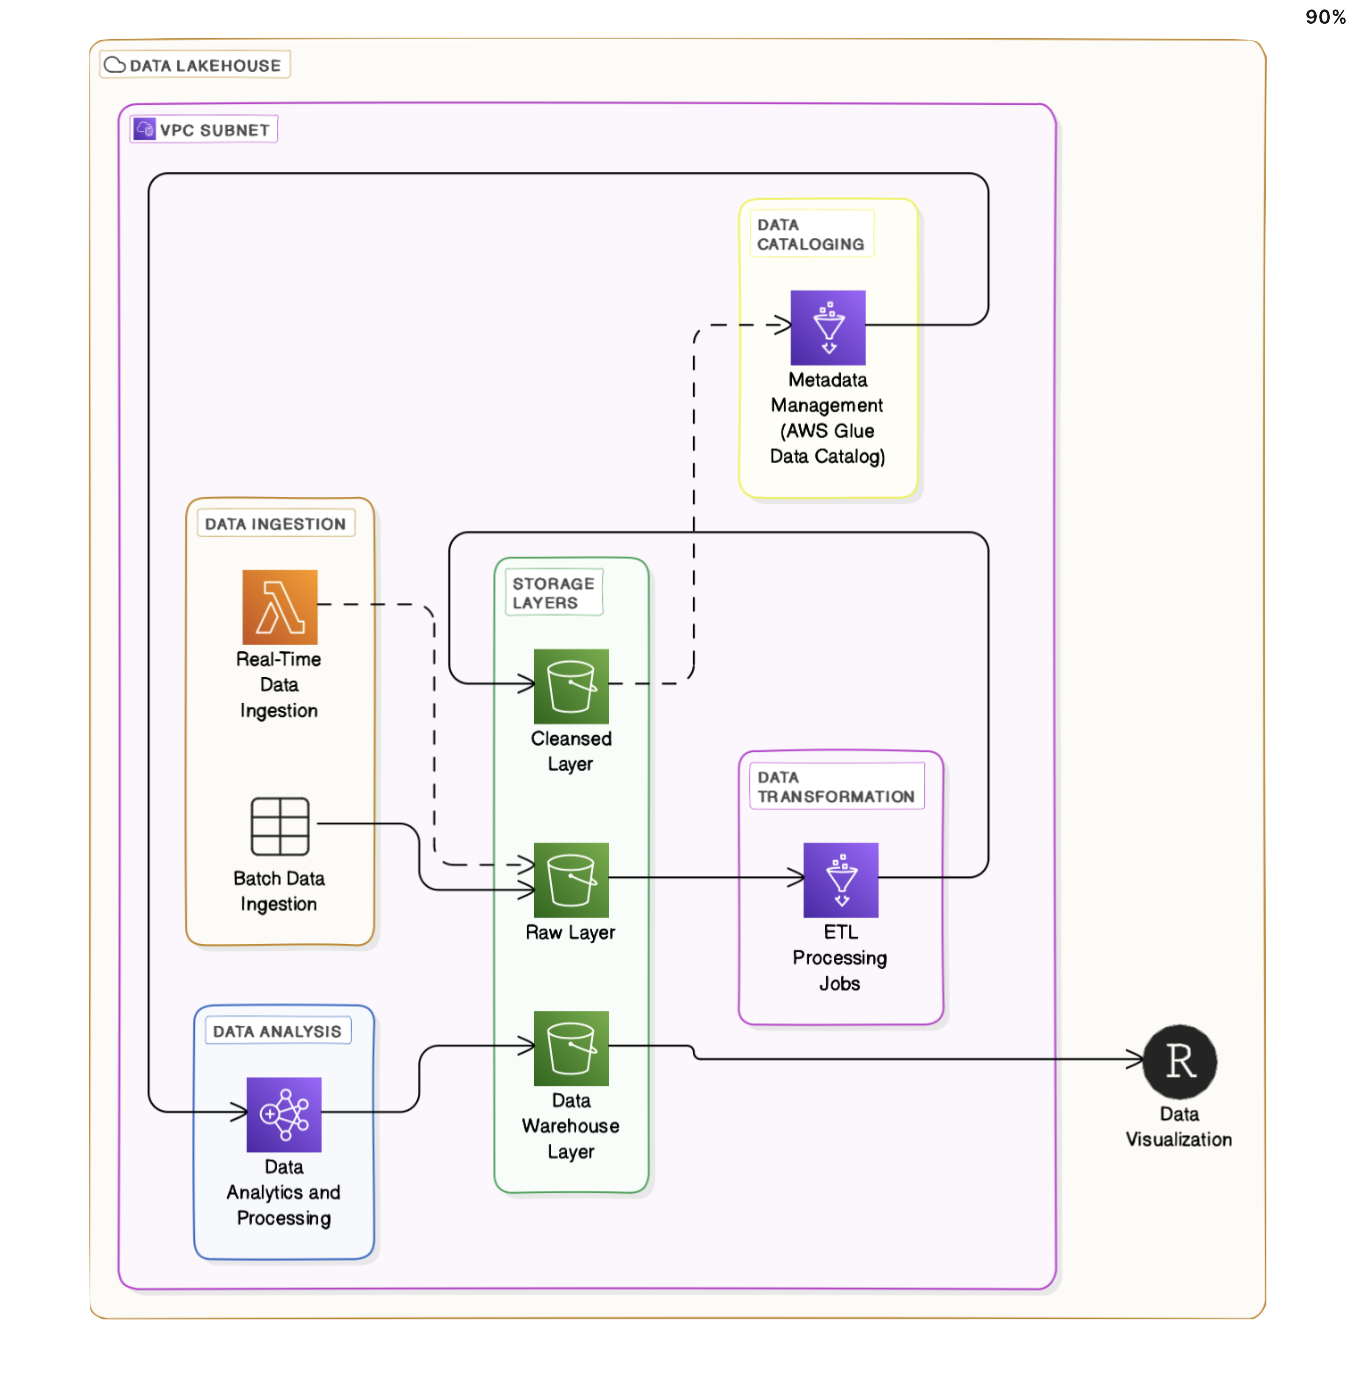
\includegraphics[width=0.8\textwidth]{images/arch/AWS-GridGuru-LakeHouseArchitecture.png}
    \caption{\textbf{AWS Data LakeHouse Architecture Diagram}}
\end{figure}

\section{Data Analysis with F1 Dataset}

We employed a dual dataset approach:

\begin{itemize}
    \item \textbf{Static Dataset:} This dataset contains historical information from past Formula 1 seasons, including data on race results, driver standings, lap times, and other relevant metrics. It was provided through our personal contacts at AWS and F1, ensuring a reliable and comprehensive foundation for our analysis with trusted and familiar data sources.
    \item \textbf{Dynamic Dataset:} This dataset provides real-time information for the current 2024 season. AWS Lambda is used to ingest this data by making API calls to gather the latest updates, ensuring that our analysis remains current with ongoing events. Here, we used OpenF1 API, Ergast API, and Formula One API (F1 Api) as data sources.
\end{itemize}
By integrating these datasets into our Data Lakehouse architecture on AWS, we effectively manage both historical and real-time data. 

The static dataset allows us to analyze trends and patterns over previous seasons, while the dynamic dataset enables us to monitor and react to live data from the current season.

Our analysis aimed to uncover actionable insights that could inform race strategies and enhance the performance of both teams and drivers. We utilized SQL queries on our Amazon EMR cluster to efficiently process and analyze the substantial data volumes. These queries were meticulously crafted to explore hypotheses regarding the relationships between various factors such as weather conditions, track characteristics, and driver performance metrics.

Upon obtaining initial results and drawing preliminary conclusions from these queries, we further refined our analysis by exporting the data to the Curated Layer in Amazon S3. These files were then imported into a dedicated workspace in RStudio for detailed visualization. This additional step allowed us to visually interpret the data more intuitively, facilitating the identification of significant patterns and trends that underpin our strategic recommendations.

\subsection{Database Structure Overview}
For our exploratory data analysis (EDA), we used a combination of historical and current datasets, structured into several tables with specific focuses. Each table captures unique aspects of the sport, allowing for a comprehensive analysis from multiple angles. Here's a brief guide to some tables:

\begin{itemize}
    \item \textbf{Circuits}: Contains details about the various circuits used in the races, including location, length, and other relevant information.
    \item \textbf{Constructor Results}: Records the results achieved by each constructor in different races, including points and status.
    \item \textbf{Constructor Standings}: Summarizes the standings of constructors throughout the season, capturing their cumulative points and positions.
    \item \textbf{Constructors}: Lists the constructors participating in a season, along with their basic information and attributes.
    \item \textbf{Driver Standings}: Details the standings of drivers across the season, showing their cumulative points and positions after each race.
    \item \textbf{Drivers}: Contains information about the drivers, including personal details, nationality, and career statistics.
    \item \textbf{Lap Times}: Records the times for each lap completed during race weekends, providing timing and performance data.
    \item \textbf{Pit Stops}: Details the pit stops made during races, including timing and duration.
    \item \textbf{Qualifying}: Captures the results of the qualifying sessions, determining the starting grid for the races.
    \item \textbf{Races}: Provides comprehensive information about each race event, including date, location, and participating drivers and constructors.
    \item \textbf{Results}: Summarizes the race results for each event, including positions, points, and other performance metrics.
    \item \textbf{Seasons}: Lists the seasons of the championship, including the year and other relevant details.
    \item \textbf{Sprint Results}: Contains the results of the sprint qualifying sessions, including grid positions and points awarded.
    \item \textbf{Status}: Describes the status of drivers in each race, such as whether they finished or the reason for not finishing.
\end{itemize}

\subsection{Query Analysis and Insights}

\subsubsection{Total Accidents by Circuit and Sector}

\paragraph{Description}
This analysis delves into the distribution of total accidents across various circuits, segmented by individual sectors. The primary goal is to identify which sections of each circuit are more prone to incidents, thereby guiding improvements in safety measures and refining race strategies.

\begin{figure}[H]
    \centering
    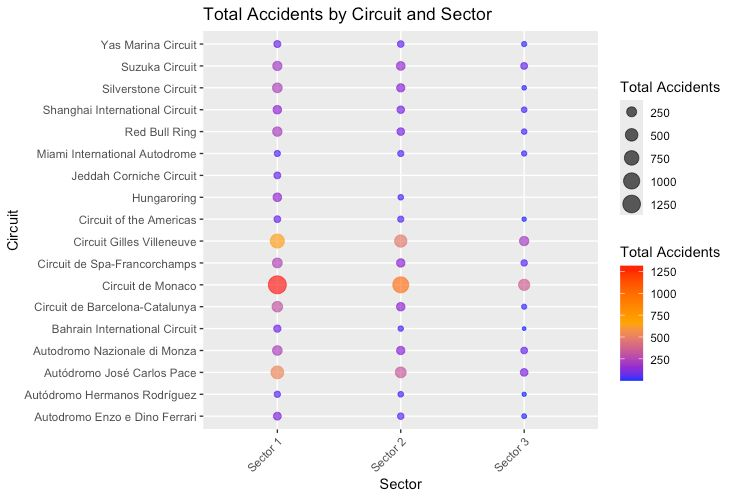
\includegraphics[width=0.8\textwidth]{images/querie/accidentsByCircuitSector.jpeg}
    \caption{Total Accidents by Circuit and Sector}
\end{figure}

\paragraph{Interpretation}
The dot plot reveals significant variability in accident distribution across the circuits. Notably, Sectors 1 and 2 of the Circuit de Monaco are highlighted as particularly dangerous, exhibiting a higher frequency of accidents. This suggests that these sectors may contain challenging track features or conditions that increase the likelihood of incidents. 

Conversely, circuits like Yas Marina and Circuit of the Americas show fewer accidents, particularly in their respective Sector 3, indicating areas where drivers possibly face fewer challenges or where track conditions are less conducive to accidents. 

This analysis is crucial for identifying which circuits require more careful attention during race preparations and which may afford a more aggressive approach. It helps us as a team to know where extra caution is necessary and where they might push the limits more safely.

\subsubsection{Performance Analysis: Average Points Per Season vs Wins}

\paragraph{Description}
This bubble chart provides a comparative analysis of Formula 1 drivers' performance, showcasing the relationship between the average points per season and total wins. The drivers are represented with bubbles, color-coded by team and sized according to the number of retirements, offering insights into both performance and reliability.

\begin{figure}[H]
    \centering
    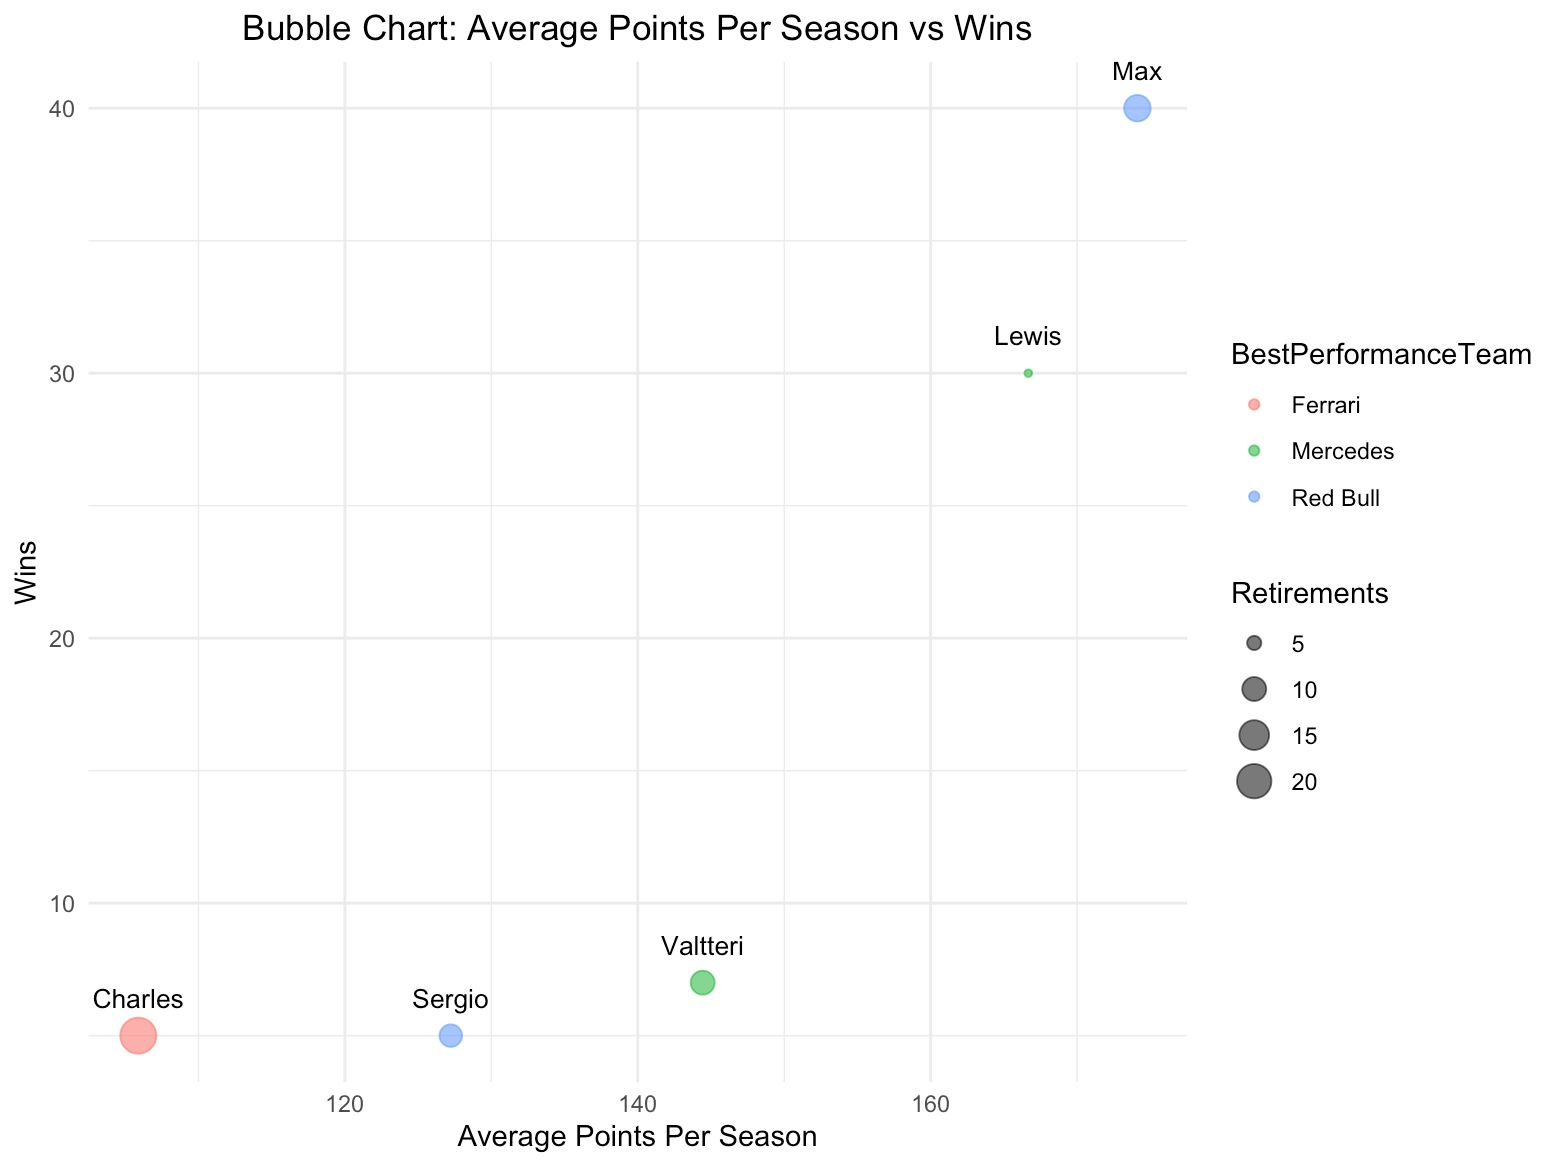
\includegraphics[width=0.8\textwidth]{images/querie/newDriver.jpeg}
    \caption{Bubble Chart: Average Points Per Season vs Wins}
\end{figure}

\paragraph{Interpretation}
The chart clearly shows that Valtteri and Sergio (Checo) exhibit similar performance levels in terms of average points per season, both positioned in the middle tier of the plot, which suggests a consistent but not top-tier performance compared to leaders like 'Max' and 'Lewis'. Both Checo and Valtteri show a solid ability to accumulate points, although Valtteri has a slightly higher win count, indicating potential in high-stakes situations.

Valtteri's performance makes him an ideal potential replacement for Checo, as his ability to secure wins under various conditions suggests he could bring additional strengths to the team. Furthermore, Valtteri's experience with a top team like Mercedes could provide valuable insights and strategies, enhancing team dynamics and performance. His positioning in the chart, coupled with fewer retirements compared to Checo, underscores his reliability and consistency, for any hypothetical replacement for Checo.

\subsubsection{Pit Stop Strategy Analysis: Average Duration vs Number of Stops}

\paragraph{Description}
This scatter plot examines the relationship between the average duration of pit stops and the total number of pit stops for each Formula 1 team. It highlights efficiency and strategic execution during races, providing a snapshot of how well teams manage their pit stop strategies.

\begin{figure}[H]
    \centering
    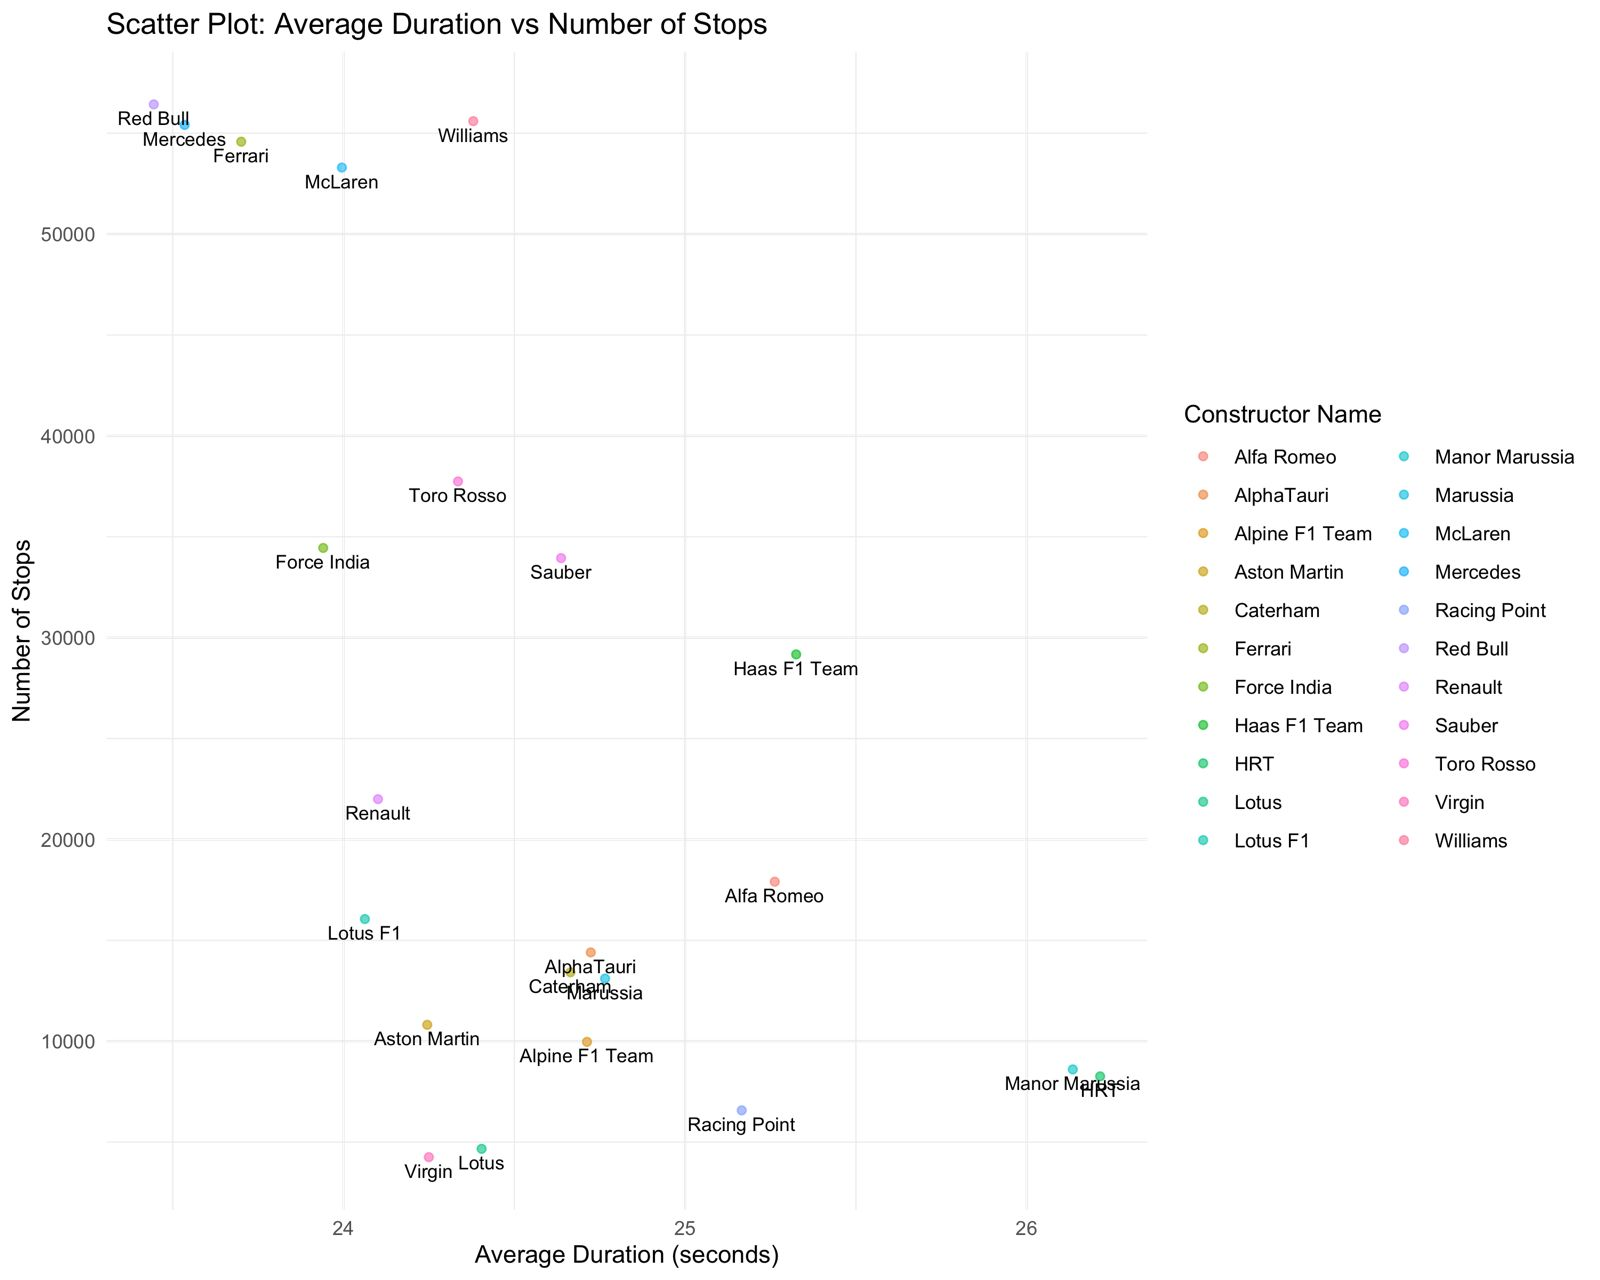
\includegraphics[width=0.82\textwidth]{images/querie/pitStopStrategy.jpeg}
    \caption{Scatter Plot: Average Duration vs Number of Stops}
\end{figure}

\paragraph{Interpretation}
The chart positions our team in the upper left quadrant, indicative of many pit stops with shorter average durations, underscoring the team's exceptional efficiency and strategic prowess in pit stop management. This placement is superior compared to main competitors like Mercedes and Ferrari, who also perform well but do not match our teams's leading position.

Given our advantageous standing in this analysis, focusing substantial resources on further reducing pit stop times may yield diminishing returns compared to other areas where performance gains could be more significant. Our team's current pit stop strategy not only demonstrates effective execution but also suggests that the existing practices are highly optimized. This efficiency in pit stops provides us with a competitive edge, allowing more flexibility in race strategies and potentially contributing to better race outcomes.

\subsubsection{Analysis of Position Change from Starting Grid to Race End for Active Drivers in 2024}

\paragraph{Description}
This scatter plot assesses the average position change from the starting grid to the race end for active Formula 1 drivers in the 2024 season. It quantifies each driver's ability to maintain or improve their position throughout a race, providing a measure of consistency and racecraft.

\begin{figure}[H]
    \centering
    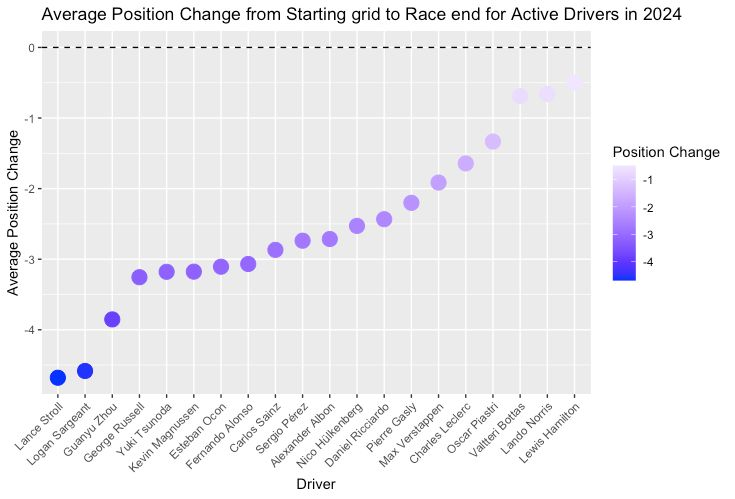
\includegraphics[width=0.95\textwidth]{images/querie/gridVSend.jpeg}
    \caption{Average Position Change from Starting Grid to Race End for Active Drivers in 2024}
\end{figure}

\paragraph{Interpretation}
The plot illustrates that most drivers tend to lose positions by the end of the race, with our drivers, Perez and Verstappen, showing different trends. Perez shows a minor position loss on average, which suggests a strong ability to defend his starting position. In contrast, Verstappen exhibits a slightly more favorable position retention, which emphasizes his skill in maintaining or slightly improving his race standing.

It is crucial to note that gaining many positions during a race, known as making a 'comeback', is not a common occurrence and typically indicates exceptional circumstances or strategies during the race. The proximity of our both drivers to zero in this metric underscores their effectiveness in maximizing race outcomes based on their starting positions. This consistent performance near the baseline suggests that while dramatic position gains are rare, the ability to maintain or slightly improve positions is a significant indicator of a driver's skill and strategic execution during races.


\subsubsection{Analysis of Circuit Danger Levels Based on Total Incidents}

\paragraph{Description}
This bar chart categorizes various Formula 1 circuits into three tiers based on the total number of incidents reported: Above Average Danger, Average Danger, and Below Average Danger. Each tier reflects the relative safety or risk of the circuits during races, providing crucial insights for team strategy and driver safety preparations.

\begin{figure}[H]
    \centering
    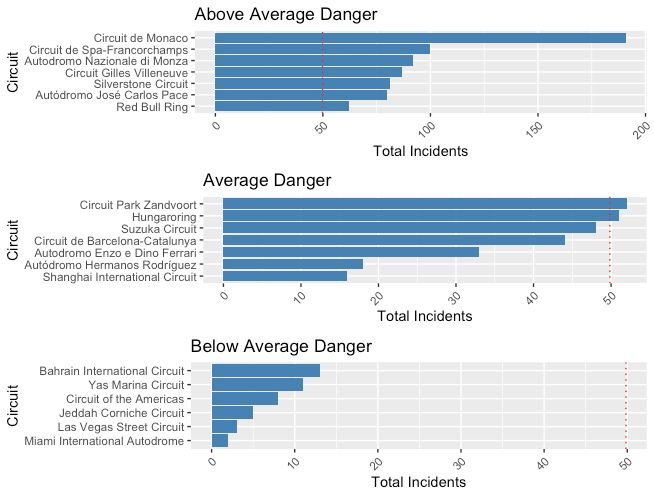
\includegraphics[width=0.7\textwidth]{images/querie/Dangerous-tracks.jpeg}
    \caption{Circuit Danger Levels Based on Total Incidents}
\end{figure}

\paragraph{Interpretation}
The chart identifies circuits with varying levels of danger. Notably, circuits like Monaco, Spa-Francorchamps, and Silverstone are in the 'Above Average Danger' category, indicating a higher frequency of incidents. These circuits, known for their challenging layouts and high-speed corners, often require more cautious approaches and robust safety strategies.

Conversely, circuits categorized under 'Below Average Danger', such as Bahrain and Yas Marina, show fewer incidents, suggesting safer conditions and potentially less challenging tracks. For our team, understanding these distinctions is crucial. While it's important to push for optimal performance, strategizing for safety and reliability at more dangerous circuits can prevent costly incidents and ensure consistent point accumulation.
For circuits with above-average danger, we might consider more conservative strategies or focus on reliability and driver safety to minimize risks. At circuits with below-average danger, there may be opportunities to be more aggressive in terms of strategy, aiming for maximum points without the heightened risk of incidents.


\subsubsection{Analysis of Reliability Issues for Red Bull and Comparison with Other Constructors}

\paragraph{Description}
This bar chart provides a comprehensive analysis of the reliability issues encountered by our team compared to the constructors with the maximum and minimum reliability issues in various categories such as accidents, brakes, engine, and gearbox problems. The chart categorizes issues to highlight areas where our team excels or faces challenges relative to other teams in Formula 1.

\begin{figure}[H]
    \centering
    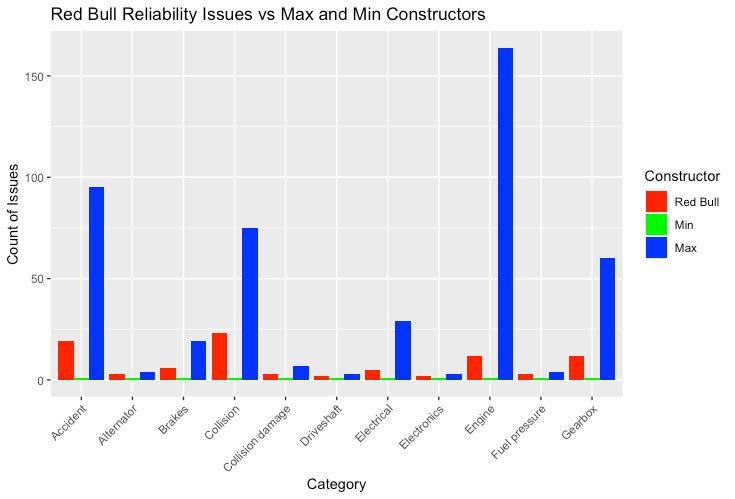
\includegraphics[width=0.8\textwidth]{images/querie/reliability.jpeg}
    \caption{Red Bull Reliability Issues vs Max and Min Constructors}
\end{figure}

\paragraph{Interpretation}
The data indicates that our team has fewer issues in several categories compared to the constructors with the maximum issues, suggesting a high level of reliability and effective management in those areas. Notably, we have fewer problems related to accidents, aerodynamics, and collision damage, reflecting a robust car design and effective risk management strategies during races. This performance underscores the overall excellence of our vehicle, indicating not only a strong technical foundation but also a testament to the skill and precision of our engineering team. The reliability across various aspects of race management shows that our car is well-suited to the demands of Formula 1 racing, consistently performing at a high level while minimizing potential disruptions during critical events.


\subsubsection{Performance Rate Analysis: Wins per Lap for Top Formula 1 Teams}

\paragraph{Description}
This bar chart evaluates the performance rate of the top Formula 1 teams by measuring wins per lap completed. This metric provides an efficiency ratio that highlights not just the number of victories, but how effectively each team converts laps into wins. It serves as a comprehensive indicator of overall team performance, integrating aspects of reliability, speed, and strategic execution.

\begin{figure}[H]
    \centering
    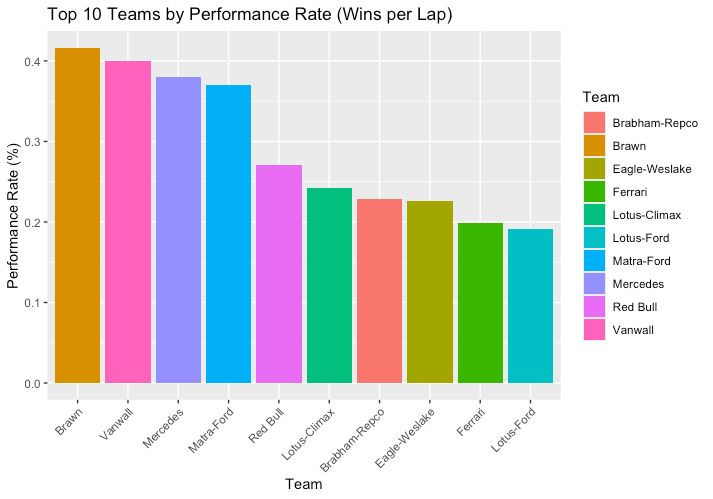
\includegraphics[width=0.8\textwidth]{images/querie/laps-vs-wins.jpeg}
    \caption{Top 10 Teams by Performance Rate (Wins per Lap)}
\end{figure}

\paragraph{Interpretation}
The chart places our team solidly in the middle of the pack, indicating a competitive but not dominant performance rate in terms of wins per lap. This suggests that while our team is efficient in translating laps into wins, there is potential for improvement compared to teams like Mercedes and Brawn, which exhibit higher efficiency. This current standing reflects a balance between consistency and the occasional brilliance needed to secure victories.


\subsubsection{Cluster Analysis of Circuits by Average Points for Our Drivers}

\paragraph{Description}
This bar chart employs the K-means clustering algorithm, a popular machine learning technique used for partitioning a dataset into K distinct, non-overlapping clusters. In this method, data points are grouped by minimizing the sum of distances between each data point and the centroid of the cluster to which it belongs. The algorithm iterates through two steps—assigning points to the nearest cluster centroid and then updating the centroid of the clusters until the centroids stabilize. This analysis categorizes Formula 1 circuits based on the average points scored by our drivers in races, illustrating the effectiveness of our team's performance across different tracks.

\begin{figure}[H]
    \centering
    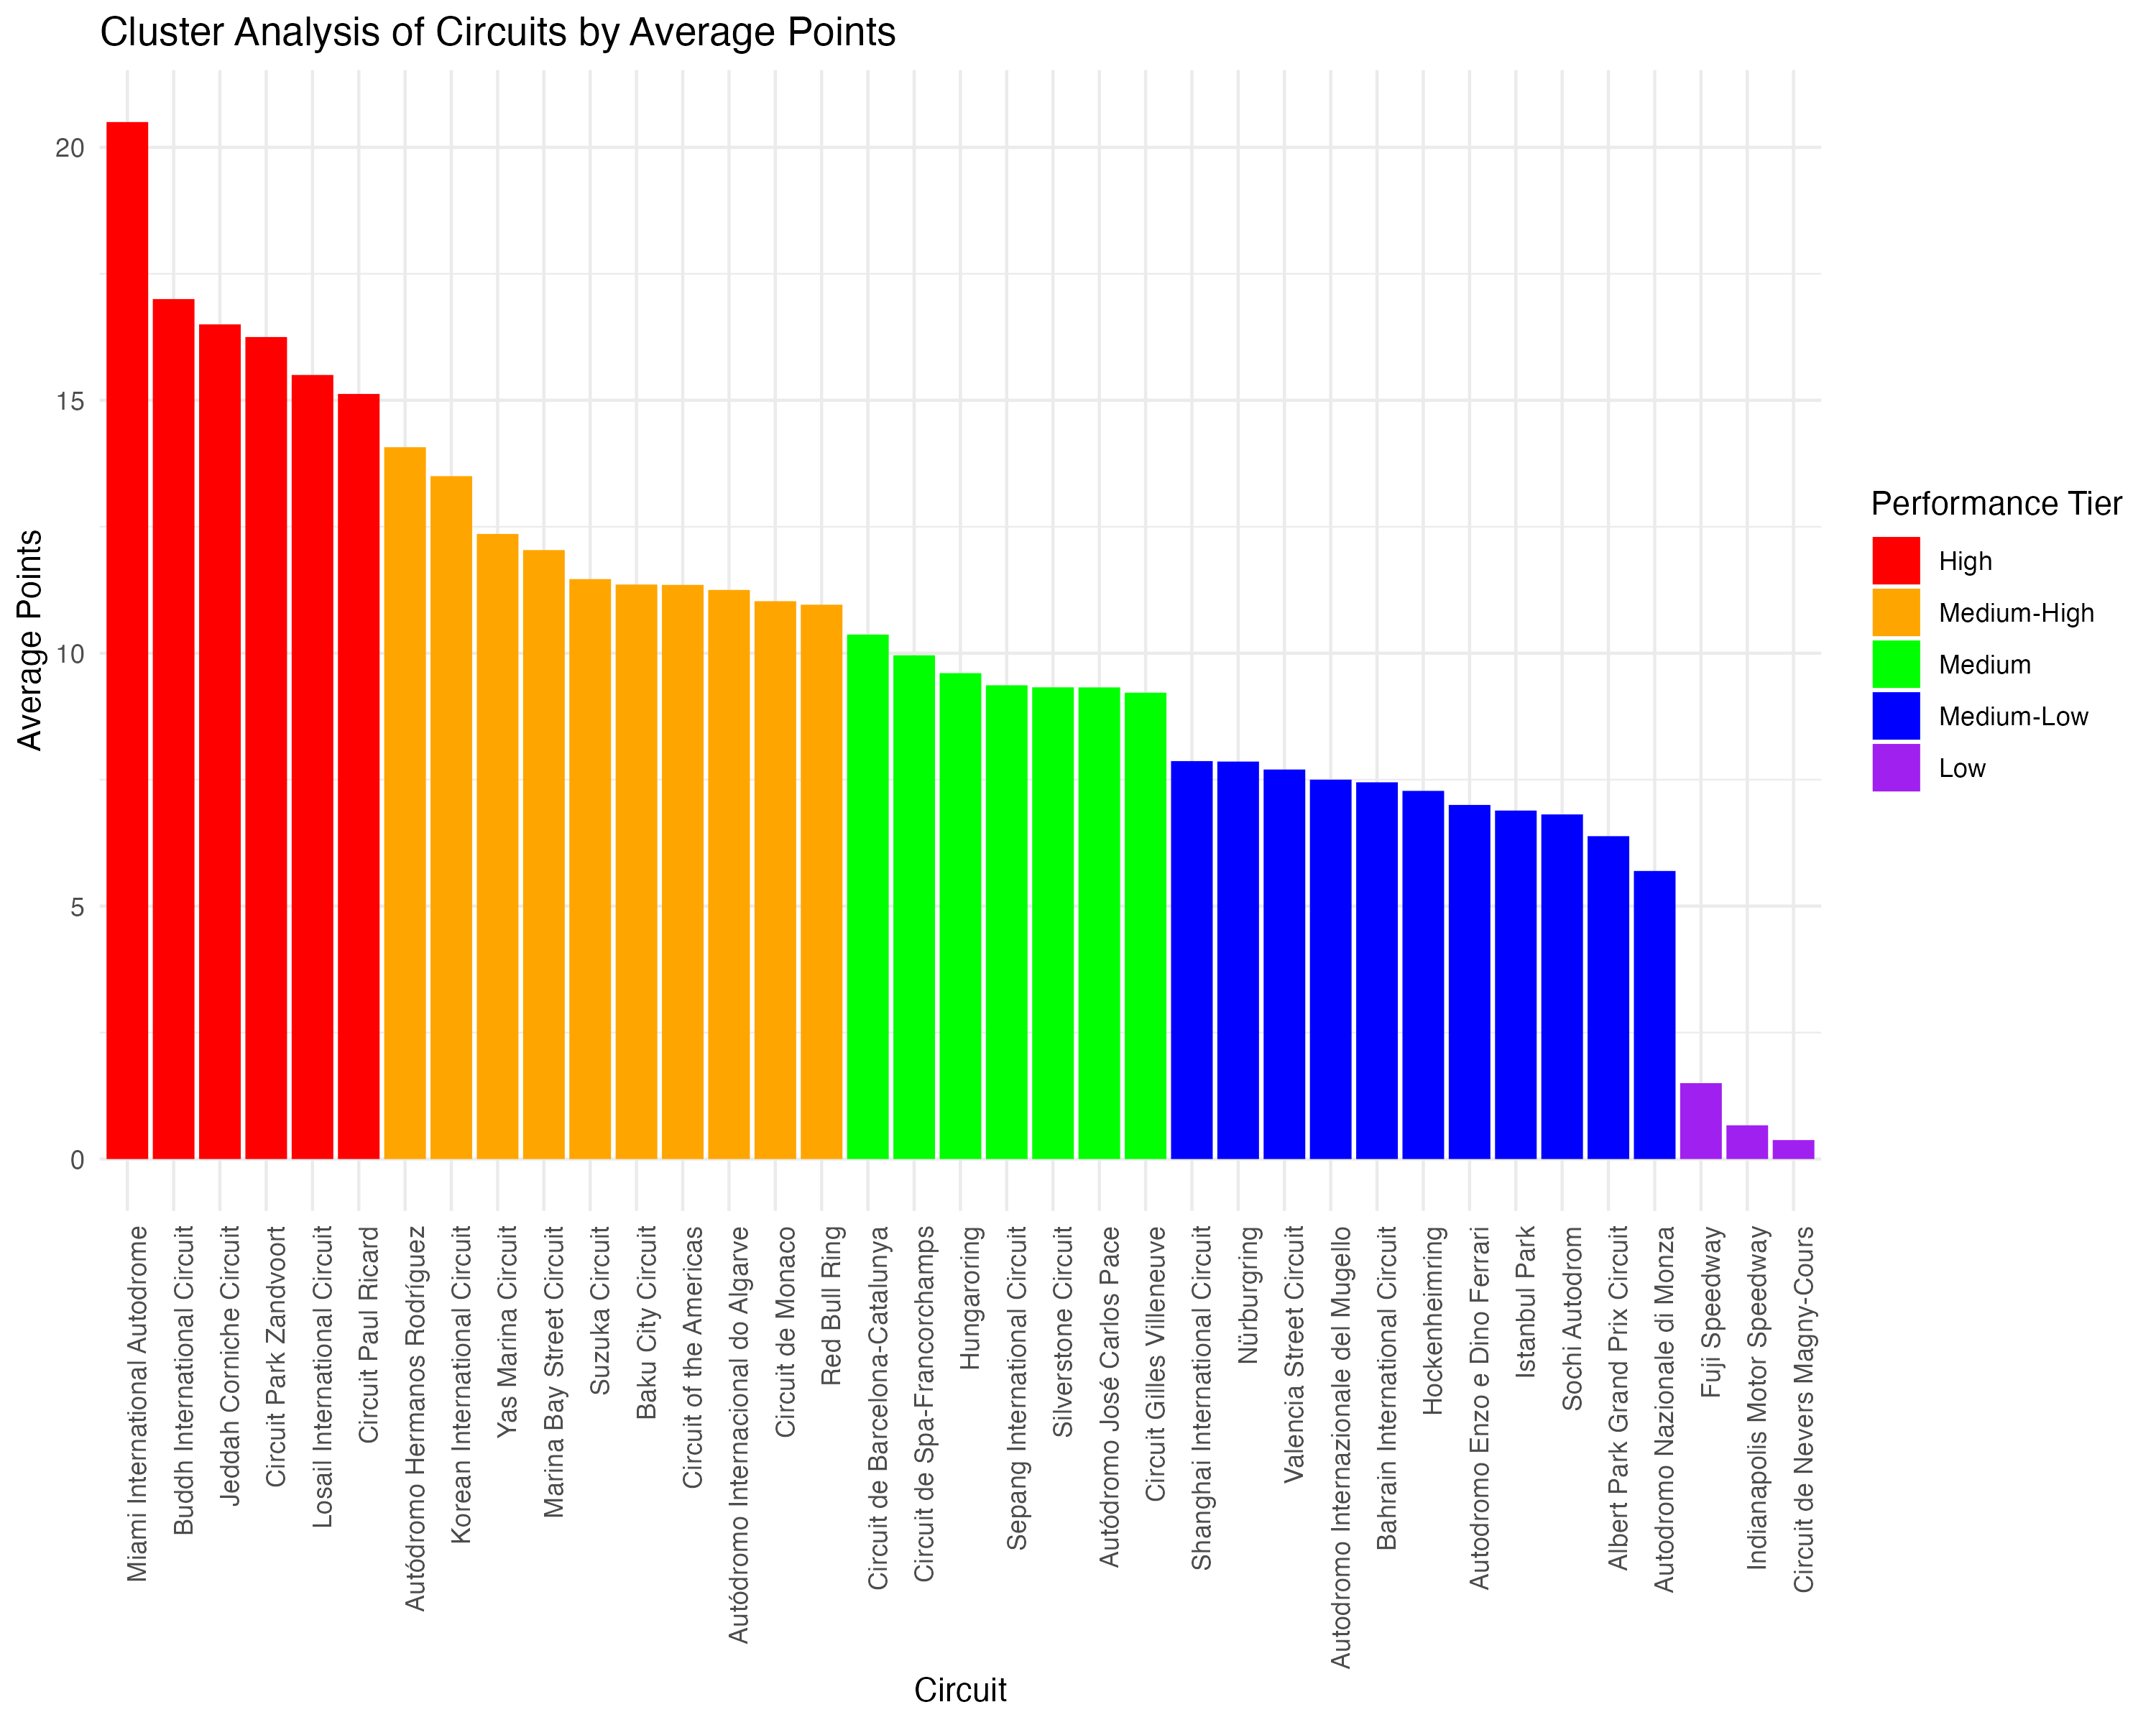
\includegraphics[width=0.68\textwidth]{images/querie/cluster_average_points_per_circuit.png}
    \caption{Cluster Analysis of Circuits by Average Points for Our Drivers}
\end{figure}

\paragraph{Interpretation}
The clusters range from 'High' performance (red) to 'Low' performance (purple) tiers, each color signifying a group of circuits where our drivers tend to score differently. High-tier circuits like Miami International Autodrome show that our drivers consistently achieve higher points, suggesting favorable conditions or a strong alignment with our car's capabilities and our drivers' skills.

Conversely, circuits categorized in the 'Low' tier, such as Las Vegas Street Circuit, are typically tougher for our drivers, indicating possible areas for further strategy refinement or potential improvements in car setup to better tackle these challenging tracks. The insights from this clustering help in understanding where our team excels and where we face challenges, guiding strategic decisions for future races.



\section{Challenges Encountered}
\subsection{Infrastructure-Related Challenges}
\paragraph{Description:}
Initially, our project was set up on Google Cloud Platform (GCP). However, we faced a significant challenge when our GCP credits were exhausted. To continue our work without interruption, we opted to create a simplified version of a Data Lakehouse on AWS. This decision was influenced by the opportunities and services available in AWS, which allowed us to replicate the necessary functionalities we initially had on GCP. We carefully selected AWS services that closely matched those we used on GCP to ensure a smooth transition and maintain the efficiency of our data processing and analysis.


\section{Conclusions}
Our analysis has provided several key insights that could significantly influence the strategic approaches of Red Bull Racing. Firstly, the reliability analysis highlights that while the team's performance is generally robust. Secondly, the cluster analysis of circuit performance by average points offers a strategic map for prioritizing resources and tactics according to the circuit characteristics. Lastly, the in-depth examination of pit stop strategies and accident data across circuits underlines the importance of tailored strategies that adapt to the nuances of each race environment. Overall, these insights not only reinforce the strengths but also address the critical areas where Red Bull Racing can gain competitive advantages, ensuring that the team remains a formidable contender in the Formula 1 championships.

\section{Project Repository}
\url{https://github.com/enriquegomeztagle/BigData/tree/main/FinalTerm/F1-GridGuru-Project}

\end{document}
